\documentclass[10pt, a4paper]{article}
% \usepackage[english]{babel}
\usepackage[brazilian]{babel}
\usepackage[utf8]{inputenc}
% \usepackage[T1]{fontenc}

% matlab code
% \usepackage{matlab-prettifier}
%\usepackage[numbered,framed]{matlab-prettifier}
\usepackage{pythonhighlight}
\renewcommand{\lstlistingname}{Anexo} % Listing->Code
\let\ph\mlplaceholder % shorter macro
\definecolor{codegreen}{rgb}{0,0.6,0}
\definecolor{codegray}{rgb}{0.5,0.5,0.5}
\definecolor{codepurple}{rgb}{0.58,0,0.82}
\definecolor{backcolour}{rgb}{0.95,0.95,0.92}
\lstdefinestyle{myStyle}{
    language=Matlab,
    breaklines=true,
    frame=single,
    numbers=none,
    basicstyle=\ttfamily\footnotesize,
%     basicstyle=\footnotesize\ttfamily,
    keywordstyle=\bfseries\color{magenta},
    commentstyle=\color{codegreen},
    identifierstyle=\color{blue},
    backgroundcolor=\color{backcolour},
    stringstyle=\color{codepurple},
}
\usepackage{adjustbox}

% For subfigure use
\usepackage[font=small,labelfont=bf]{caption}
\usepackage{subcaption}

% Set page size and margins
% Replace `letterpaper' with`a4paper' for UK/EU standard size
\usepackage[a4paper,top=2cm,bottom=2cm,left=2cm,right=2cm,marginparwidth=2cm]{geometry}

% tabelas
\usepackage{array}
\usepackage{tabularx}
\usepackage{booktabs}

\usepackage{float}

% Useful packages
\usepackage{amsmath}

\usepackage{graphicx}
%\graphicspath{{figures/}} %Setting the graphicspath
\usepackage[colorlinks=true, allcolors=blue]{hyperref}
\usepackage{cleveref}
\newcommand{\crefrangeconjunction}{--}


\begin{document}

\def\TITLE{Lista 00}
\def\DISCIPLINE{MEC 2403 - Otimização e Algoritmos para Engenhria Mecânica}
\def\PROFESSOR{Ivan Menezes}
\def\AUTHOR{Pedro Henrique Cardoso Paulo}
\def\CONTACT{pedrorjpaulo.phcp@gmail.com}
\def\DATE{março de 2023}

\title{\textbf{\TITLE} \\ \DISCIPLINE}
\author{\AUTHOR}
\date{\DATE}

\begin{titlepage}
      \begin{center}
          \vspace*{1cm}

          \Huge
          \textbf{\TITLE}

          \vspace{0.5cm}
          \LARGE
          \DISCIPLINE

          \vspace{1.5cm}

          \textbf{\AUTHOR \\ {\tt \CONTACT}}

          \vfill
          Professor: \PROFESSOR

          \vspace{0.8cm}

          
\includegraphics[width=0.2\textwidth]{../general/puc.jpg}

          \Large
          Departamento de Engenharia Mecânica\\
          PUC-RJ Pontifícia Universidade Católica do Rio de Janeiro\\
          \DATE

      \end{center}
  \end{titlepage}

\maketitle

\section{Introdução}

\subsection{Objetivos}

Esse é o entregável da \TITLE \ da disciplina \DISCIPLINE. Esse trabalho tem como objetivos:

\begin{enumerate}
  \item Fixar os conceitos de gradiente e matriz Hessiana, com um exemplo
  \item Fixar o conceito de matriz positiva definida, com um exemplo
  \item Trabalhar a ideia de aproximação de uma função por polinômios de Taylor
  \item Trabalhar a ideia de parametrização de uma reta por vetor e projeção de funções em seu plano
  \item Exercitar o uso de ferramentas computacionais para visualização de funções
\end{enumerate}

\subsection{Links úteis}\label{links}

Nesta seção são listados alguns links e referências úteis para se entender o trabalho desempenhado.

\begin{enumerate}
  \item \href{https://web.tecgraf.puc-rio.br/~ivan/MEC2403/ProgMatematica_VazPereiraMenezes-Ago2012.pdf}{Apostila de programação matemática da disciplina}
  \item \href{https://github.com/prj-phcp/MEC2403_Activities}{GitHub usado para essa disciplina}
  \item \href{https://github.com/prj-phcp/MEC2403_Activities/blob/master/Lista0/Lista0.ipynb}{Notebook com o código para as figuras desse relatório}
\end{enumerate}

\section{Questão 01}

\subsection{Enunciado}

Calcular o gradiente e a matriz Hessiana da função $f(x_1, x_2, x_3)$, dada pela equação \cref{q01:en}

\begin{equation}\label{q01:en}
  f(x_1, x_2, x_3) = 3x_1^3x_2^2x_3 - 6x_1x_3^4\log{x_2} + x_1^{-1}x_2^3 - x_1^2\sqrt{x_2}
\end{equation}

onde $\log{x}$ reprersenta o logaritmo neperiano.

\subsection{Solução}

A expressão para o gradiente ($\nabla f$) e para a Hessiana ($\mathbf{H}$) são apresentadas, respectivamente, nas equações \cref{q01:grad} e \cref{q01:hess}

\begin{equation}\label{q01:grad} 
  \nabla f =
  \left[ {\begin{array}{c}
    \frac{\partial f}{\partial x_1} \\
    \frac{\partial f}{\partial x_2} \\
    \frac{\partial f}{\partial x_3} \\
  \end{array} } \right]
\end{equation}

\begin{equation}\label{q01:hess} 
  \mathbf{H} =
  \left[ {\begin{array}{ccc}
    \frac{\partial^2 f}{\partial x_1^2} & \frac{\partial^2 f}{\partial x_1x_2} & \frac{\partial^2 f}{\partial x_1x_3} \\
    \frac{\partial^2 f}{\partial x_1x_2} & \frac{\partial^2 f}{\partial x_2^2} & \frac{\partial^2 f}{\partial x_2x_3} \\
    \frac{\partial^2 f}{\partial x_1x_3} & \frac{\partial^2 f}{\partial x_2x_3} & \frac{\partial^2 f}{\partial x_1^2} \\
  \end{array} } \right]
\end{equation}

Vale ressaltar que a formulação da Hessiana já faz uso do da igualdade matemática de derivadas segundas expressa na equação \cref{q01:teo}

\begin{equation}\label{q01:teo}
  \frac{\partial^2 f}{\partial x_i x_j} = \frac{\partial^2 f}{\partial x_j x_i}
\end{equation}

Dessa forma, o problema da determinação do gradiente e da hessiana se resume ao problema do cálculo das derivadas de primeira 
e seunda ordem da função $f(x_1, x_2, x_3)$. Começando pelas derivadas de primeira ordem para determinação do gradiente, estas são 
expressas pelas equações \cref{q01:dx1,q01:dx2,q01:dx3}

\begin{equation}\label{q01:dx1}
    \frac{\partial f}{\partial x_1} = 9x_1^2x_2^2x_3 - 6x_3^4\log{x_2} - x_1^{-2}x_2^3 - 2x_1\sqrt{x_2}
\end{equation}

\begin{equation}\label{q01:dx2}
    \frac{\partial f}{\partial x_2} = 6x_1^3x_2x_3 - 6x_1x_2^{-1}x_3^4 + 3x_1^{-1}x_2^2 - \frac{x_1^2}{2\sqrt{x_2}}
\end{equation}

\begin{equation}\label{q01:dx3}
    \frac{\partial f}{\partial x_3} = 3x_1^3x_2^2 - 24x_1x_3^3\log{x_2}
\end{equation}

Já as derivadas segundas, necessárias para a determinação da Hessiana, são dadas pelas equações 
\cref{q01:dx1x1,q01:dx2x2,q01:dx3x3,q01:dx1x2,q01:dx1x3,q01:dx2x3}

\begin{equation}\label{q01:dx1x1}
    \frac{\partial^2 f}{\partial x_1^2} = 18x_1x_2^2x_3 + 2x_1^{-3}x_2^3 - 2\sqrt{x_2}
\end{equation}

\begin{equation}\label{q01:dx2x2}
    \frac{\partial^2 f}{\partial x_2^2} = 6x_1^3x_3 + 6x_1x_2^{-2}x_3^4 + 6x_1^{-1}x_2 + \frac{x_1^2}{4x_2\sqrt{x_2}}
\end{equation}

\begin{equation}\label{q01:dx3x3}
    \frac{\partial^2 f}{\partial x_3^2} = - 72x_1x_3^2\log{x_2}
\end{equation}

\begin{equation}\label{q01:dx1x2}
    \frac{\partial^2 f}{\partial x_1x_2} = 18x_1^2x_2x_3 - 6x_2^{-1}x_3^4 - 3x_1^{-2}x_2^2 - \frac{x_1}{\sqrt{x_2}}
\end{equation}

\begin{equation}\label{q01:dx1x3}
    \frac{\partial^2 f}{\partial x_1x_3} = 9x_1^2x_2^2 - 24x_3^3\log{x_2}
\end{equation}

\begin{equation}\label{q01:dx2x3}
    \frac{\partial^2 f}{\partial x_2x_3} = 6x_1^3x_2 - 24x_1x_2^{-1}x_3^3
\end{equation}



\section{Questão 02}

\subsection{Enunciado}

Classificar a matriz abaixo quanto à sua positividade:

\[
  \mathbf{A} =
  \left[ {\begin{array}{ccc}
     3 & -2 &  1 \\
    -2 &  4 & -3 \\
     1 & -3 &  2 \\
  \end{array} } \right]
\]

\subsection{Solução}

A determinação da positividade da matriz será feita por meio de seus autodeterminantes. 
Caso os 3 autodeterminantes da matriz sejam positivos, sabe-se que ela será positiva definida (ou semi-definida caso algum seja zero). 
Caso eles alternem entre valores positivos e negativos, sabe-se que ela será negativa definida. Caso contrário,
nada pode-se afirmar. Calculando o primeiro:

\[
  \left| {\begin{array}{c}
    3\\
  \end{array} } \right| = 3
\]

Calculando o segundo:

\[
  \left| {\begin{array}{cc}
     3 & -2 \\
    -2 &  4 \\
  \end{array} } \right| = 8
\]

Calculando o terceiro:

\[
  \left| {\begin{array}{ccc}
     3 & -2 &  1 \\
    -2 &  4 & -3 \\
     1 & -3 &  2 \\
  \end{array} } \right| = -3
\]

Como nenhum dos padrões descritos foi respeitado, a matriz não é nem 
positiva definida e nem negativa definida, 
ou seja, a matriz apresenta autovalores positivos e negativos.


\section{Questão 03}\label{q03}

\subsection{Enunciado}

Determinar a expansão em série de Taylor, em torno do ponto $x = 1$, 
da função $f(x) = e^{2x}$. Em seguida, usando o MATLAB ou Python, 
plotar os gráficos da função $f$ e de suas respectivas aproximações
(polinômios) de ordens 0, 1, 2 e 3.

\subsection{Solução}

Para a função em questão, suas derivadas são calculadas de acordo com a regra de 
derivação da função exponencial. Assim temos que a derivada n-ésima da função 
$f(x)$ criada é dada pela equação \cref{q03:deriv}

\begin{equation}\label{q03:deriv}
    \frac{d^nf}{dx^n} = 2^n e^{2x}
\end{equation}

Pela definição da série de Taylor, para uma expansão ao redor de $x = 1$, temos 
que a expansão da função seria a dada pela equação \cref{q03:taylor}

\begin{equation}\label{q03:taylor}
    f(x) \cong \sum^{\infty}_{n=0} 2^n e^2 (x-1)^n
\end{equation}

O primeiro passo é implementar em Python as funções {\tt f} e {\tt taylor\_f} que 
representam, respectivamente, a função f definida na questão e seu polinômio 
de Taylor de ordem arbitrária.

\begin{python}
def f(x):

return np.exp(2*x)

def taylor_f(x, order):

f_approx = 0
for n in range(order+1):
    f_approx += (x-1)**n * (2**n) * np.exp(2)
return f_approx
\end{python}

As funçoes são implementadas com funções do módulo 
{\tt numpy} de modo a garantir a vetorização. Uma vez tendo as funções implementadas,
podemos plotar gráficos das aproximações desejadas parta vizinhanças dos ponto $x = 1$
usando o seguinte código:

\begin{python}
orders = [0, 1, 2, 3] # Ordens da aproximacao
points = 50 # Pontos de x considerados
x_min = 0 # Minimo x
x_max = 2 # Maximo x
x_values = np.linspace(x_min, x_max, points)
fig, ax = plt.subplots(1,1, figsize=(5, 5))
f_real = f(x_values)
ax.plot(x_values, f_real, 'm--', label='$f(x) = e^{2x}$')
for n in orders:
    f_approx = taylor_f(x_values, n)
    ax.plot(x_values, f_approx, label=f'ordem = {n}')

ax.plot(1, f(1), 'ko')
ax.legend()
ax.grid()
\end{python}

A \cref{fig:q3} apresenta alguns plots com diferentes intervalos de $x$ para a análise
da aporximação dos polinômios de Taylor. É possível ver que, para ordens maiores, a aproximação
tente a ficar melhor na vizinhança do ponto expandido, mas isso não necessariamente é verdade 
conforme nos afastamos dele.

\begin{figure}
    \centering
    \begin{subfigure}[b]{0.32\textwidth}
        \centering
        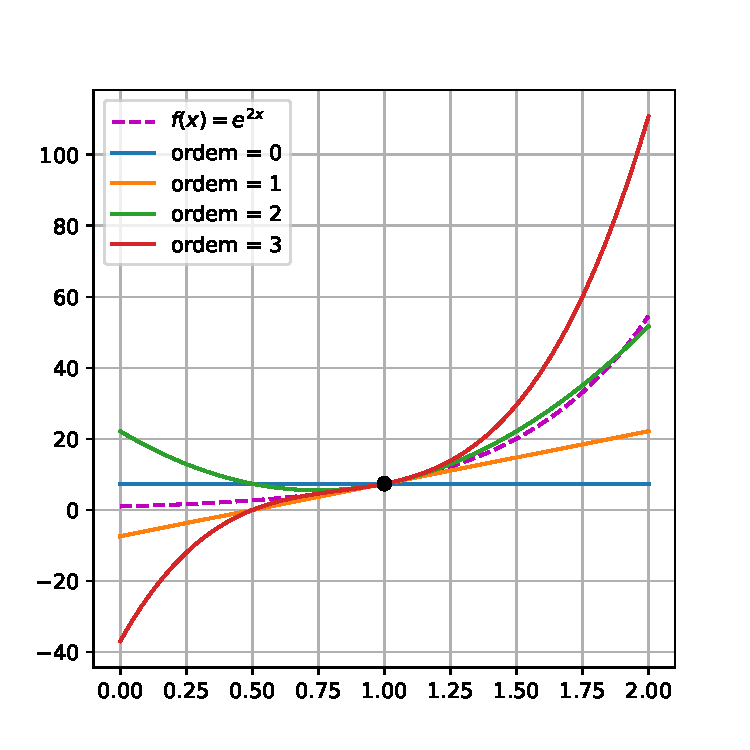
\includegraphics[width=\textwidth]{images/q3_1.pdf}
        \caption{$x \in [0, 2]$}
        \label{fig:q3_1}
    \end{subfigure}
    \hfill
    \begin{subfigure}[b]{0.32\textwidth}
        \centering
        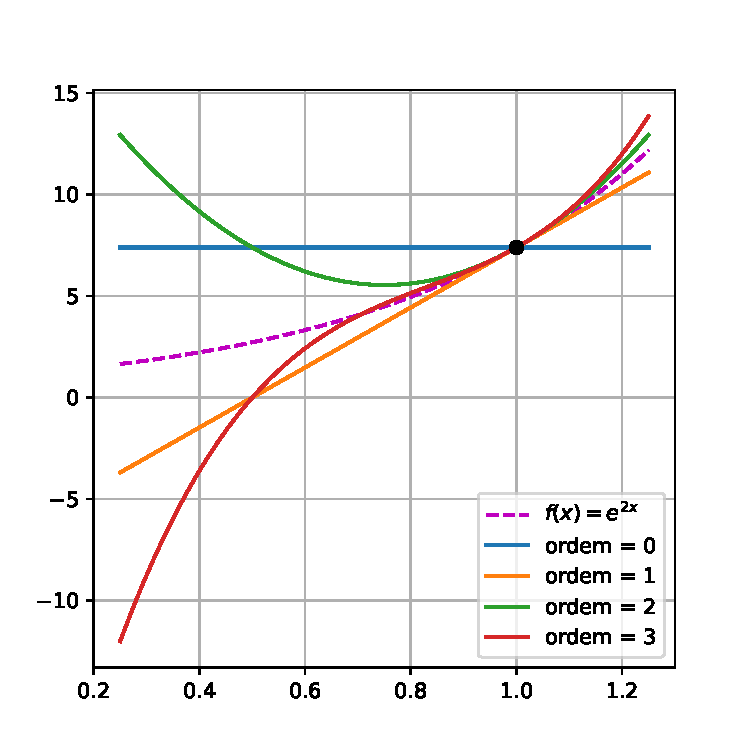
\includegraphics[width=\textwidth]{images/q3_2.pdf}
        \caption{$x \in [0.25, 1.25]$}
        \label{fig:q3_2}
    \end{subfigure}
    \hfill
    \begin{subfigure}[b]{0.32\textwidth}
        \centering
        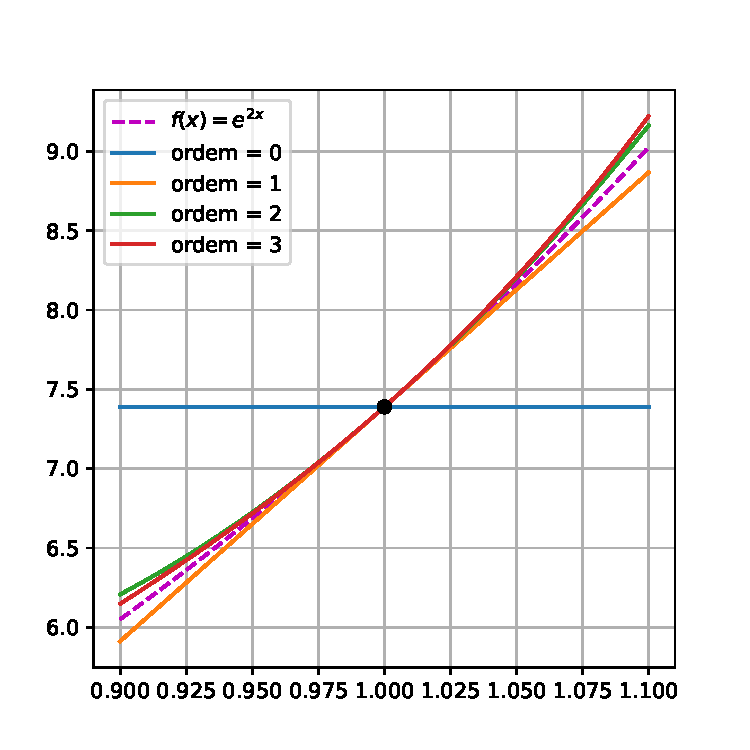
\includegraphics[width=\textwidth]{images/q3_3.pdf}
        \caption{$x \in [0.9, 1.1]$}
        \label{fig:q3_3}
    \end{subfigure}
       \caption{Função $f(x) = e^{2x}$ e seus polinômios de Taylor}
       \label{fig:q3}
\end{figure}

\newpage

\section{Questão 04}

\subsection{Enunciado}

Seja a função $f(x_1, x_2)$ dada pela equação \cref{q04:func}

\begin{equation}\label{q04:func}
    f(x_1, x_2) = x_1^3 + 2x_1 x_2^2 - x_2^3 - 20x_1
\end{equation}

Desenhar o gráfico da curva contida em um plano Cartesiano, 
cujo eixo das abscissas corresponde à reta que passa pelos pontos 
$P_1 = (-0.7, 1.6)$ e $P_2 = (3.7,-0.4)$, a origem desse eixo é no 
ponto $P_1$ e o eixo das ordenadas corresponde aos valores da função $f$. 
Utilizar o MATLAB ou Python e considerar apenas o trecho entre os pontos 
$P_1$ e $P_2$.

\subsection{Solução}

De forma similar ao feito na Questão 03 (seção \ref{q03}), nossa solução começa por meio da
implementação da função Python que representa a equação que desejamos estudar. Essa função receberá
um vetor 1D que tem as coordenadas do ponto no plano $xy$.

\begin{python}
def f2(P):
    return P[0]**3 + 2*P[0]*(P[1]**2) - P[1]**3 - 20*P[0]
\end{python}

A determinação da equação da reta que passa pelos pontos $P_1$ e $P_2$, por sua vez, será feita
vetorialmente por meio da equação paramétrica \cref{q04:reta}

\begin{equation}\label{q04:reta}
  \mathbf{P} = \mathbf{P_1} + \alpha\mathbf{\hat{v}}, \quad \alpha \in \left[0, ||\mathbf{v}||\right]
\end{equation}

onde o vetor $\mathbf{v} = \mathbf{P_2} - \mathbf{P_1}$. É importante notar que, 
no espaço 3D, essa reta determina, na verdade, um plano paralelo ao eixo vertical,
de modo que o objetivo da questão é determinar a interseção entre esse plano e a superfície
definida na equação \cref{q04:func}. Em Python, o plot dessa interseção pode ser feito por meio do seguinte código:

\begin{python}
P1 = np.array([-0.7, 1.6])
P2 = np.array([3.7, -0.4])
v = P2 - P1
v_norm = np.linalg.norm(v)
v_hat  = v / v_norm

points = 50
x_values = np.linspace(0, v_norm, points)
y_values = f2(P1.reshape(-1,1) + v_hat.reshape(-1,1)*x_values.reshape(1,-1))
fig, ax = plt.subplots(1,1, figsize=(5, 5))
ax.plot(x_values, y_values, 'm--', label='Funcao projetada')
ax.hlines(0, 0, v_norm, 'k', linewidth=1.0)
ax.set_xlim(0, v_norm)
ax.plot(0, 0, 'ko')
ax.text(0.05, -2.5, '$P_1$')
ax.plot(v_norm, 0, 'ko')
ax.text(4.6, -2.5, '$P_2$')
ax.legend()
ax.grid()
\end{python}

A visualização 2D dessa interseção, junto com uma representação 3D do problema é apresentada na 
\cref{fig:q4}. Para mais informações sobre o código para a visualização 3D, visite o Notebook 
referenciado na seção \ref{links}. A execução deste Notebook permite também a interação com o 
gráfico, com rotação e mudança do ponto de visualização 3D.


\begin{figure}
    \centering
    \begin{subfigure}[b]{0.45\textwidth}
        \centering
        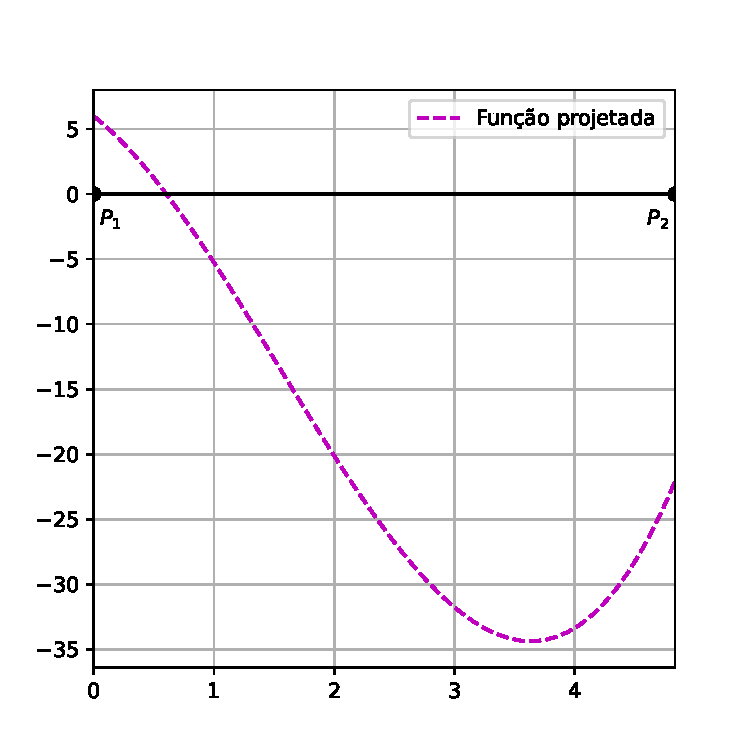
\includegraphics[width=\textwidth]{images/q4_1.pdf}
        \caption{Visão 2D}
        \label{fig:q4_1}
    \end{subfigure}
    \hfill
    \begin{subfigure}[b]{0.5\textwidth}
        \centering
        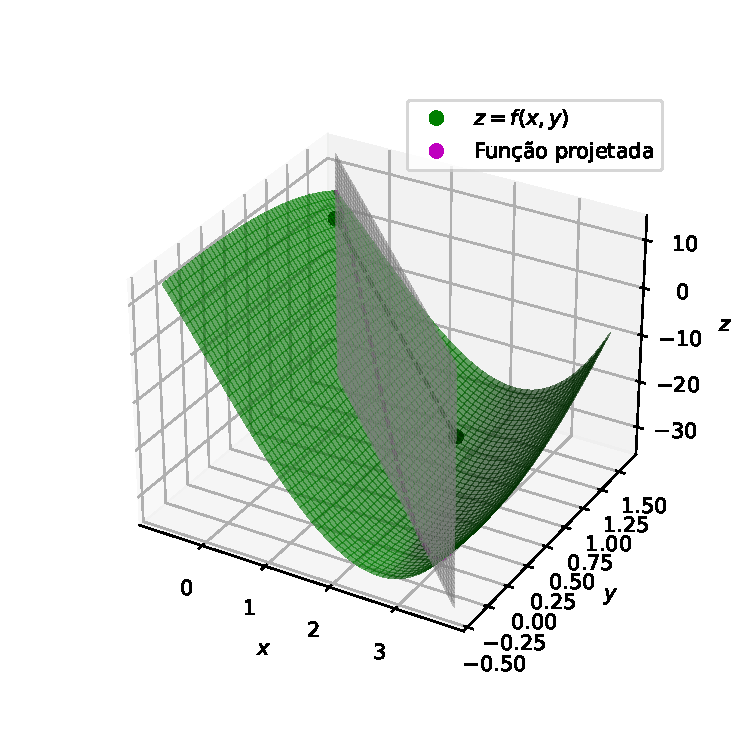
\includegraphics[width=\textwidth]{images/q4_2.pdf}
        \caption{Visão 3D}
        \label{fig:q4_2}
    \end{subfigure}
    \hfill
       \caption{Plot da projeção da função no plano da reta}
       \label{fig:q4}
\end{figure}



\bibliographystyle{apalike}
\bibliography{export}

\end{document}